%*****************************************************************************************
%*********************************** Second Chapter **************************************
%*****************************************************************************************

\chapter{Methods}

\ifpdf
    \graphicspath{{Chapter2/Figs/Raster/}{Chapter2/Figs/PDF/}{Chapter2/Figs/}}
\else
    \graphicspath{{Chapter2/Figs/Vector/}{Chapter2/Figs/}}
\fi



\section{Petri Nets}
\subsection{Syntax and Semantics of Basic nets}
A Petri Net is a 4-tuple $(P, T, pre, post)$ defined as:
\begin{itemize}
\item[-] a set of \textit{places} (or conditions) $P$
\item[-] a set of \textit{transitions} (or events) $T$
\item[-] a \textit{preconditions map pre} : $T \rightarrow \mathbf{m}P$ which assigns a multiset of places $pre(t)$ to each transition $t \in T$
\item[-] a \textit{postconditions map post} : $T \rightarrow \mathbf{m}P$ which assigns a multiset of places $post(t)$ to each transition $t \in T$
\end{itemize}
where $\mathbf{m}P$ is the space of multisets over $P$ with a multiset over P defined as function $f: P \rightarrow \mathbb{N}$. The state of the system, called a marking, is again a multiset $\mathcal{M}$ over $P$. We can think of the marking as the distributed global state of the system. It is also common when defining a Petri Net to give the initial marking of the system usually written as $\mathcal{M}_0$.

The operational semantics of Petri Nets is defined in terms of changes in the global state through the action of 
the transitions $T$ of the PN:
\begin{equation*}
\mathcal{M}\overset{t}{\longrightarrow}\mathcal{M^\prime}
\end{equation*}
Here when a transition(event) $t$ occurs it changes the state of the system from marking $\mathcal{M}$ to marking $\mathcal{M^\prime}$. Unlike automata and Turing Machines however a transition does not occur from a single global state but instead it only affects part of the state:
\begin{equation*}
\mathcal{M}\overset{t}{\longrightarrow}\mathcal{M^\prime} \mbox{ iff } pre(t) \leq \mathcal{M} \mbox{ and } \mathcal{M^\prime} = \mathcal{M} - pre(t) + post(t)
\end{equation*}
For 2 multisets $f$ and $g$ over set $X$, $f \leq g$ is defined as $f \leq g \iff \forall x \in X f_x \leq g_x$. So a transition $t$ is said to be 'enabled' if its preconditions are sufficiently marked($pre(t) \leq \mathcal{M}$) and when it 'fires' it changes the marking in the places in its vicinity, namely the set of places $\{p \mbox{ }|\mbox{ } pre(t)_p \neq 0 \mbox{ or } post(t)_p \neq 0\}$($\mathcal{M^\prime} = \mathcal{M} - pre(t) + post(t)$). 
The \textit{post} and \textit{pre} condition maps define the causal independence between transitions and add the ability of Petri Nets to model concurrency and non-determinism. Two (or more) transitions are concurrent if they do not share any preconditions. Non-determinism is added through dependencies of transitions which share preconditions. In that case a race condition is created because the dependent transitions compete at their shared preconditions with only one of them being able to fire at each step. 

This formal definition of transitions leads to an algorithm for the executions of a PN as follows:
\begin{enumerate}[noitemsep]
\item Initialise the net  with $(P, T, pre, post)$ and set state $\mathcal{M} = \mathcal{M}_0$
\item Find enabled transitions, $enabled \subseteq T, \forall t \in T \mbox{ if } pre(t) \leq M$
\item Choose transition $t$ from set of enabled at random
\item Update state according to $\mathcal{M} = \mathcal{M} -pre(t) + post(t)$
\item Repeat steps 2-4 until there are no more enabled transitions or an external stop condition is met(e.g. max number of steps)
\end{enumerate}

The main strength of Petri Nets though lies on their very intuitive and widely used graphical representation. Petri Nets are represented as bipartite graphs with two sets of nodes, the places $P$ and transitions $T$ which are denoted by circles and rectangles respectively. A weighted directed edge with weight $n>0$ is added between place $p$ and transition $t$ in the direction $p\rightarrow t$ if $pre(t)_p=n$. A weighted directed edge with weight $n>0$ is added between transition $t$ and place $p$ in the direction $t\rightarrow p$ if $post(t)_p=n$. The markings are denoted as dots (tokens) in the circles depicting the places. So for example consider the net with $P=\{p1, p2, p3\}$, $T=\{t1\}$, $pre=\{(t1, \{(p1, 2), (p2, 1), (p3, 0)\})\}$, $post=\{(t1, \{(p1, 0), (p2, 0), (p3, 2)\})\}$, and marking $\{(p1, 3), (p2, 1), (p3, 1)\}$. The graphical depiction of this net would be the one shown in Figure \ref{fig:pn_example}. We could then also define the pre-places of a transition $t$ as all the places $p$ such that $pre(t)_p >0 $ and the post-places as all the places $p$ such that $post(t)_p >0 $.

\begin{figure}
\centering
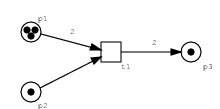
\includegraphics[scale=1.0]{pn_example}
\caption{Small basic Petri Net example}
\label{fig:pn_example}
\end{figure}

The operational semantics of Petri Nets can also be defined very naturally in this graphical notation. When a transition $t$ fires $pre(t)_p$ tokens are consumed from all the pre-places $p$ and $post(t)_p$ tokens are added to all the post-places $p$. For the net given above(Figure \ref{fig:pn_example}) when transition $t1$ fires the 2 tokens are removed from $p1$ and 1 from $p2$ and 2 are added to $p3$(see Figure \ref{fig:pn_operation}).The execution of the net can be seen as the flow of tokens through the net as transitions fire at each step according to the execution algorithm given above. This graphical view of the execution is called the 'token game' and it is very useful for gaining an insight into the dynamic behaviour of the system being modelled.
\begin{figure}
\centering
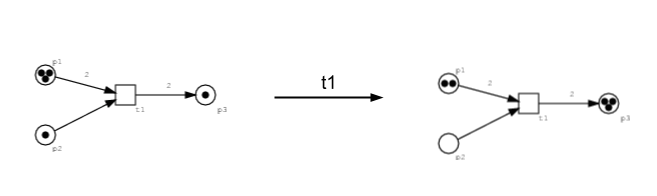
\includegraphics[scale=0.7]{pn_operation}
\caption{The token game for basic Petri Nets.}
\label{fig:pn_operation}
\end{figure}

\subsection{Stochastic Petri Net extension}
Stochastic Petri Nets are an extension to the original Petri Net formalism to explicitly model time. Notice that
even though the there is an ordering of transitions implied by their execution according to the algorithm given 
in the previous section the concept of time is not modelled explicitly in the basic Petri Net formalism. In order
to model time explicitly Stochastic Petri Nets (SPNs) introduce a waiting time associated with each transition $t$, defined as random variable $X_t$ distributed exponentially with potentially marking-dependent rate $\lambda_t(pre\_places(t))$ where $pre\_places$ is defined as before. Formally a SPN is a 5-tuple $(P, T, pre, post, \nu)$ with everything defined as before with the addition of the map $\nu : T \rightarrow H$ where $H$ is the set of all hazard functions $H = \{h_t\mbox{ }|\mbox{ } h_t: \mathbb{N}^{|pre(t)|} \rightarrow \mathbb{R}\}$.
Hazard function is the typical name used in stochastic processes for the function giving the rate of the exponential time variable. In this case the hazard function $h_t$ gives $\lambda_t$ and the domain of $h_t$ we will restrict to only the marking of the pre-places of $t$. This wait time associated with each transition changes the execution algorithm for Petri Nets; now when more than one transition is enabled a wait time is sampled from all of them and the one with the least waiting time gets to fire:
\begin{enumerate}[noitemsep]
\item Initialise the net  with $(P, T, pre, post, \nu)$, set state $\mathcal{M} = \mathcal{M}_0$, and $time=0$
\item Find enabled transitions, $enabled \subseteq T, \forall t \in T \mbox{ if } pre(t) \leq M$
\item For each enabled transition $t$ sample a wait time from an exponential distribution with rate $\lambda_t(pre\_places(t))$. Pick the transition $t_i$ with least wait time to fire.
\item Proceed time $time = time + \tau_i$
\item Update state according to $\mathcal{M} = \mathcal{M} -pre(t_i) + post(t_i)$
\item Repeat steps 2-4 until there are no more enabled transitions or an external stop condition is met(e.g. max number of steps)
\end{enumerate}
With this new variant of Petri Nets we maintain the non-determinism through the competition of enabled transitions with shared preconditions but by changing their rates we can favour some transitions over others. This Stochastic Petri Net formulation gives rise to Continuous Time Markov Chain and the execution algorithm defined above is more or less the Gillespie algorithm which is an exact algorithm for simulation of Markov jump processes. It is this Petri Net variant that we will use to model our system of interest, the Fatty Acid synthesis/elongation pathway. In the next section we describe the correspondence between a biochemical network and especially a metabolic pathway to a Stochastic Petri Net and some examples of previous uses of SPNs in biology/biochemistry.
\subsection{Application to Biochemistry}
The correspondence between a biochemical system and a Stochastic Petri Net is as follows: the chemical species of the system become places, reactions become transitions and their rates the rates of the transitions, and the stoichiometry of the reactions is represented in the \textit{pre} and \textit{post} maps. This is a very natural correspondence between chemical reactions and Petri Nets. In fact the standard notation for chemical notation is itself a process algebra albeit not a very formal one. So for example consider a made-up reaction that takes 2 molecules of A and 3 molecules of B and produces 5 molecules of C:
\begin{equation*}
2A + 3B \overset{r_k}{\longrightarrow} 5C
\end{equation*}

This is an event, a reaction with rate $k$, which tells us how the state of the system changes but although implicitly we know the conditions for it to take place they are not formally captured by the informal process algebra of chemical reactions as defined by the standard arrow notation. A Petri Net representation of this reaction however captures the reaction more formally:


\section{Stochastic Pi-calculus}
This is going to contain a vey brief introduction to stochasic pi-calculus.